\documentclass{standalone}
\usepackage{tikz}
\usetikzlibrary{patterns, positioning}
\usepackage[sfdefault]{ClearSans} %% option 'sfdefault' activates Clear Sans as the default text font
\usepackage[T1]{fontenc}

\begin{document}
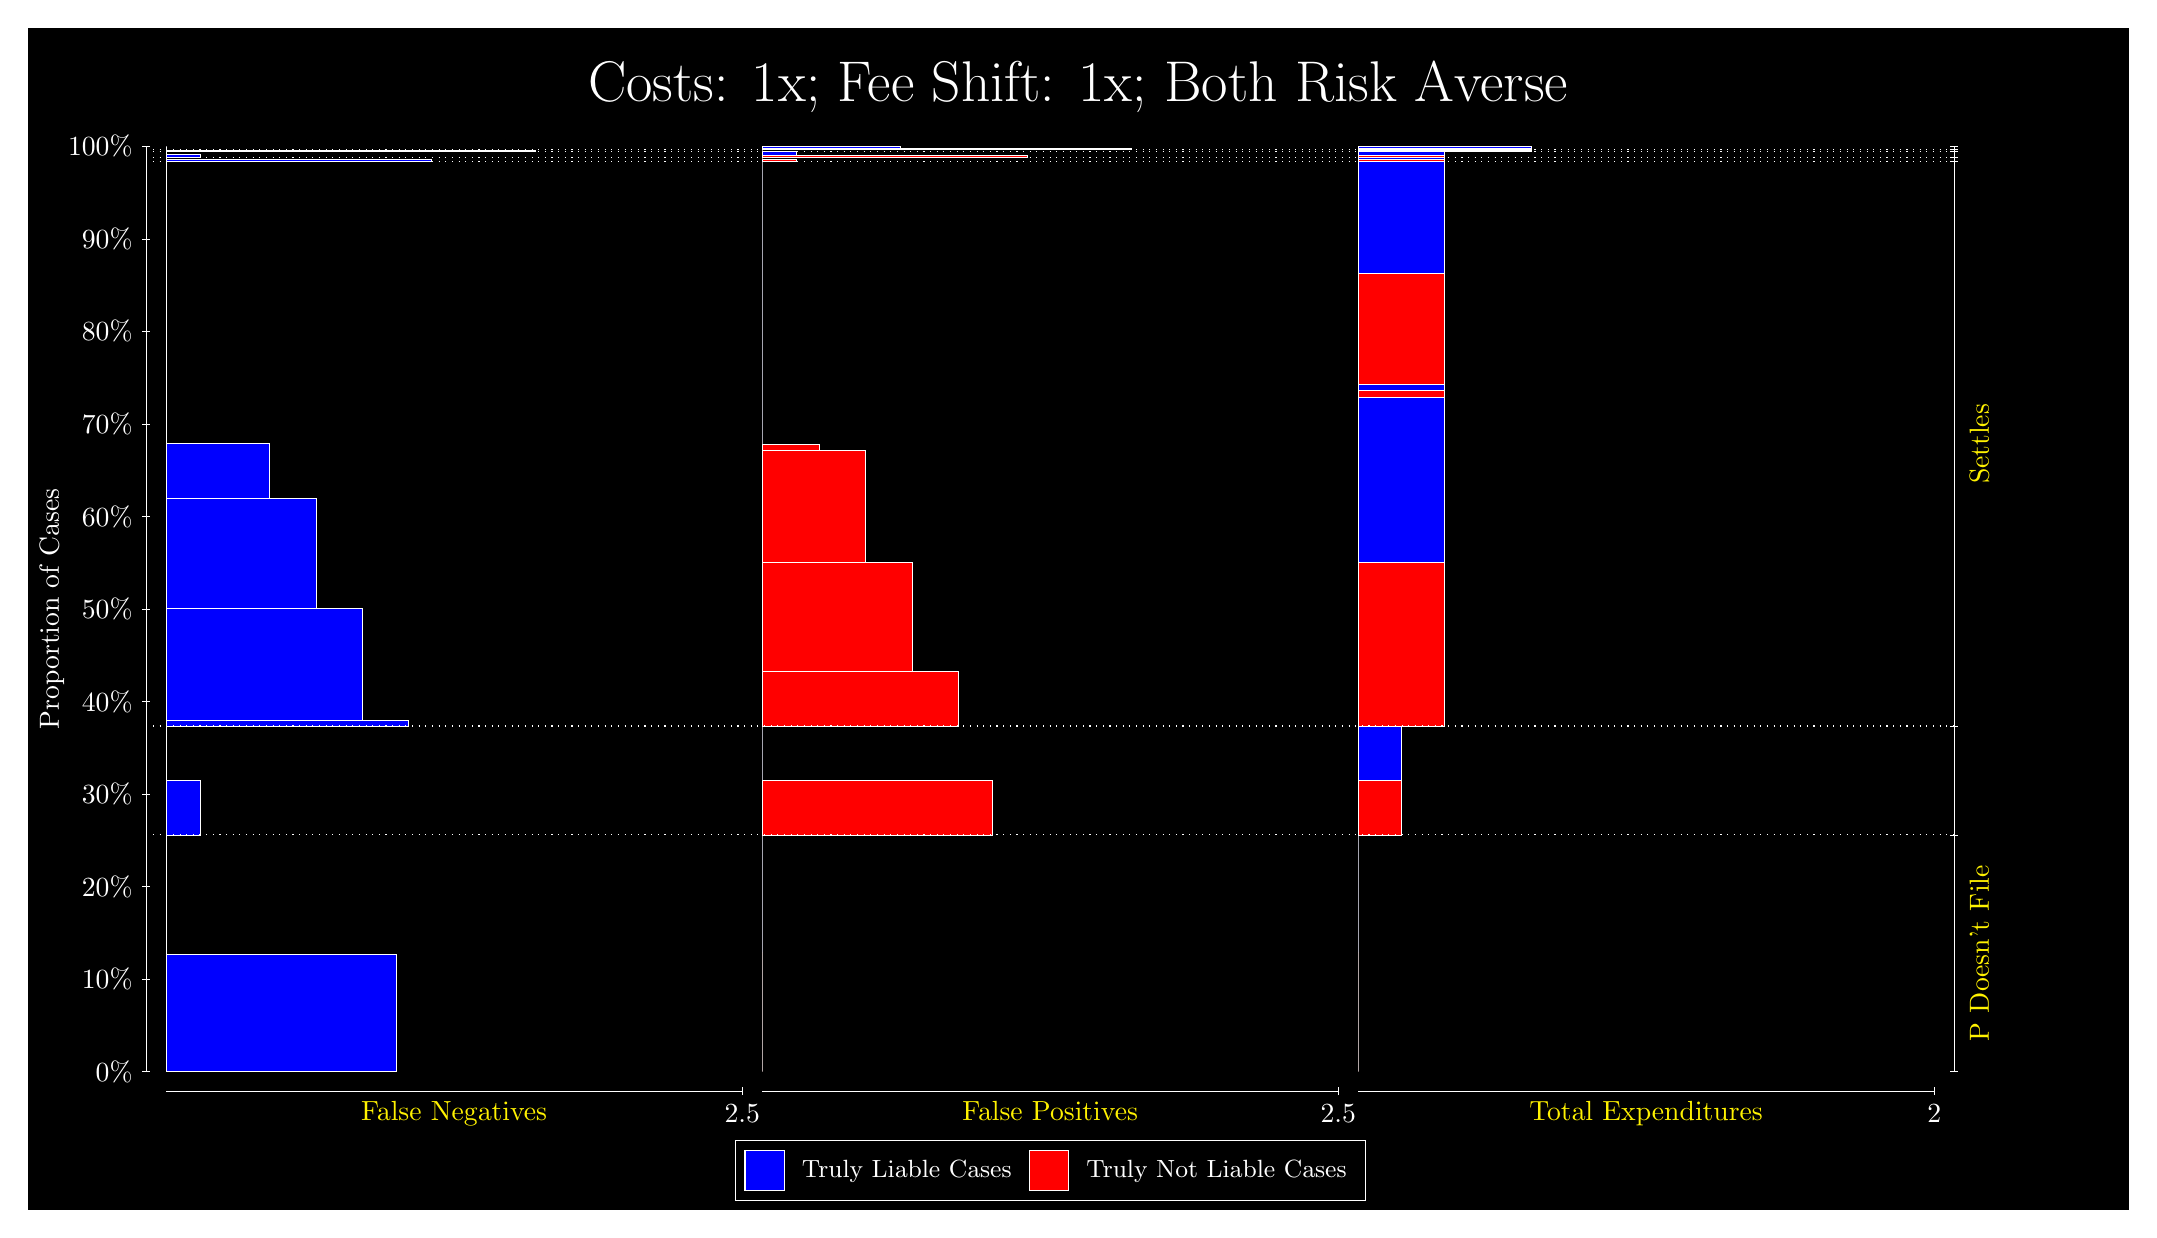
\begin{tikzpicture}
\draw[fill=black] (0,0) rectangle (26.667,15);
\draw[text=white] (0,13.5) rectangle (26.667,15) node[midway] {\huge Costs: 1x; Fee Shift: 1x; Both Risk Averse};
\draw[white, very thin] (1.5,1.75) -- (1.5,13.5);
\node[rotate=90, text=white, anchor=center] at (0.3, 7.625) {Proportion of Cases};
\draw[white, very thin] (1.45,1.75) -- (1.55,1.75);
\node[text=white, anchor=east] at (1.45, 1.75) {0\%};
\draw[white, very thin] (1.45,2.925) -- (1.55,2.925);
\node[text=white, anchor=east] at (1.45, 2.925) {10\%};
\draw[white, very thin] (1.45,4.1) -- (1.55,4.1);
\node[text=white, anchor=east] at (1.45, 4.1) {20\%};
\draw[white, very thin] (1.45,5.275) -- (1.55,5.275);
\node[text=white, anchor=east] at (1.45, 5.275) {30\%};
\draw[white, very thin] (1.45,6.45) -- (1.55,6.45);
\node[text=white, anchor=east] at (1.45, 6.45) {40\%};
\draw[white, very thin] (1.45,7.625) -- (1.55,7.625);
\node[text=white, anchor=east] at (1.45, 7.625) {50\%};
\draw[white, very thin] (1.45,8.8) -- (1.55,8.8);
\node[text=white, anchor=east] at (1.45, 8.8) {60\%};
\draw[white, very thin] (1.45,9.975) -- (1.55,9.975);
\node[text=white, anchor=east] at (1.45, 9.975) {70\%};
\draw[white, very thin] (1.45,11.15) -- (1.55,11.15);
\node[text=white, anchor=east] at (1.45, 11.15) {80\%};
\draw[white, very thin] (1.45,12.325) -- (1.55,12.325);
\node[text=white, anchor=east] at (1.45, 12.325) {90\%};
\draw[white, very thin] (1.45,13.5) -- (1.55,13.5);
\node[text=white, anchor=east] at (1.45, 13.5) {100\%};

\draw[white, very thin] (24.457,1.75) -- (24.457,13.5);
\draw[white, very thin] (24.407,1.75) -- (24.507,1.75);
\node[anchor=west] at (24.407, 1.75) {};
\draw[white, very thin] (24.407,4.7556) -- (24.507,4.7556);
\node[anchor=west] at (24.407, 4.7556) {};
\draw[white, very thin] (24.407,6.1379) -- (24.507,6.1379);
\node[anchor=west] at (24.407, 6.1379) {};
\draw[white, very thin] (24.407,13.305) -- (24.507,13.305);
\node[anchor=west] at (24.407, 13.305) {};
\draw[white, very thin] (24.407,13.361) -- (24.507,13.361);
\node[anchor=west] at (24.407, 13.361) {};
\draw[white, very thin] (24.407,13.431) -- (24.507,13.431);
\node[anchor=west] at (24.407, 13.431) {};
\draw[white, very thin] (24.407,13.465) -- (24.507,13.465);
\node[anchor=west] at (24.407, 13.465) {};
\draw[white, very thin] (24.407,13.5) -- (24.507,13.5);
\node[anchor=west] at (24.407, 13.5) {};

\draw[white, very thin, fill=blue] (1.75,1.75) rectangle (4.6775,3.2404);
\draw[white, very thin, fill=red] (1.75,3.2404) rectangle (1.75,4.7556);
\draw[white, very thin, fill=blue] (1.75,4.7556) rectangle (2.1891,5.4467);
\draw[white, very thin, fill=red] (1.75,5.4467) rectangle (1.75,6.1379);
\draw[white, very thin, fill=blue] (1.75,6.1379) rectangle (4.8239,6.2151);
\draw[white, very thin, fill=blue] (1.75,6.2151) rectangle (4.2384,7.6347);
\draw[white, very thin, fill=blue] (1.75,7.6347) rectangle (3.6529,9.033);
\draw[white, very thin, fill=blue] (1.75,9.033) rectangle (3.0674,9.7242);
\draw[white, very thin, fill=red] (1.75,9.7242) rectangle (1.75,13.305);
\draw[white, very thin, fill=blue] (1.75,13.305) rectangle (5.1167,13.333);
\draw[white, very thin, fill=red] (1.75,13.333) rectangle (1.75,13.361);
\draw[white, very thin, fill=blue] (1.75,13.361) rectangle (2.1891,13.403);
\draw[white, very thin, fill=red] (1.75,13.403) rectangle (1.75,13.431);
\draw[white, very thin, fill=blue] (1.75,13.431) rectangle (6.4341,13.448);
\draw[white, very thin, fill=red] (1.75,13.448) rectangle (1.75,13.465);
\draw[white, very thin, fill=red] (1.75,13.465) rectangle (1.75,13.48);
\draw[white, very thin, fill=blue] (1.75,13.48) rectangle (1.75,13.5);
\draw[white, very thin, fill=red] (9.3189,1.75) rectangle (9.3189,3.2652);
\draw[white, very thin, fill=blue] (9.3189,3.2652) rectangle (9.3189,4.7556);
\draw[white, very thin, fill=red] (9.3189,4.7556) rectangle (12.246,5.4467);
\draw[white, very thin, fill=blue] (9.3189,5.4467) rectangle (9.3189,6.1379);
\draw[white, very thin, fill=red] (9.3189,6.1379) rectangle (11.807,6.8291);
\draw[white, very thin, fill=red] (9.3189,6.8291) rectangle (11.222,8.2227);
\draw[white, very thin, fill=red] (9.3189,8.2227) rectangle (10.636,9.6346);
\draw[white, very thin, fill=red] (9.3189,9.6346) rectangle (10.051,9.7182);
\draw[white, very thin, fill=blue] (9.3189,9.7182) rectangle (9.3189,13.305);
\draw[white, very thin, fill=red] (9.3189,13.305) rectangle (9.758,13.333);
\draw[white, very thin, fill=blue] (9.3189,13.333) rectangle (9.3189,13.361);
\draw[white, very thin, fill=red] (9.3189,13.361) rectangle (12.686,13.389);
\draw[white, very thin, fill=blue] (9.3189,13.389) rectangle (9.758,13.431);
\draw[white, very thin, fill=red] (9.3189,13.431) rectangle (9.3189,13.448);
\draw[white, very thin, fill=blue] (9.3189,13.448) rectangle (9.3189,13.465);
\draw[white, very thin, fill=red] (9.3189,13.465) rectangle (14.003,13.48);
\draw[white, very thin, fill=blue] (9.3189,13.48) rectangle (11.075,13.5);
\draw[white, very thin, fill=red] (16.888,1.75) rectangle (16.888,3.2652);
\draw[white, very thin, fill=blue] (16.888,3.2652) rectangle (16.888,4.7556);
\draw[white, very thin, fill=red] (16.888,4.7556) rectangle (17.437,5.4467);
\draw[white, very thin, fill=blue] (16.888,5.4467) rectangle (17.437,6.1379);
\draw[white, very thin, fill=red] (16.888,6.1379) rectangle (17.986,8.2227);
\draw[white, very thin, fill=blue] (16.888,8.2227) rectangle (17.986,10.312);
\draw[white, very thin, fill=red] (16.888,10.312) rectangle (17.986,10.396);
\draw[white, very thin, fill=blue] (16.888,10.396) rectangle (17.986,10.473);
\draw[white, very thin, fill=red] (16.888,10.473) rectangle (17.986,11.885);
\draw[white, very thin, fill=blue] (16.888,11.885) rectangle (17.986,13.305);
\draw[white, very thin, fill=red] (16.888,13.305) rectangle (17.986,13.333);
\draw[white, very thin, fill=blue] (16.888,13.333) rectangle (17.986,13.361);
\draw[white, very thin, fill=red] (16.888,13.361) rectangle (17.986,13.389);
\draw[white, very thin, fill=blue] (16.888,13.389) rectangle (17.986,13.431);
\draw[white, very thin, fill=red] (16.888,13.431) rectangle (19.083,13.448);
\draw[white, very thin, fill=blue] (16.888,13.448) rectangle (19.083,13.465);
\draw[white, very thin, fill=red] (16.888,13.465) rectangle (19.083,13.48);
\draw[white, very thin, fill=blue] (16.888,13.48) rectangle (19.083,13.5);
\draw[white, dotted] (1.5,4.7556) -- (24.457,4.7556);
\draw[white, dotted] (1.5,6.1379) -- (24.457,6.1379);
\draw[white, dotted] (1.5,13.305) -- (24.457,13.305);
\draw[white, dotted] (1.5,13.361) -- (24.457,13.361);
\draw[white, dotted] (1.5,13.431) -- (24.457,13.431);
\draw[white, dotted] (1.5,13.465) -- (24.457,13.465);
\draw[white, very thin] (1.75,1.5) -- (9.0689,1.5);
\node[text=yellow, anchor=north] at (5.4094, 1.5) {False Negatives};
\draw[white, very thin] (9.0689,1.45) -- (9.0689,1.55);
\node[text=white, anchor=north] at (9.0689, 1.45) {2.5};

\draw[white, very thin] (9.3189,1.5) -- (16.638,1.5);
\node[text=yellow, anchor=north] at (12.978, 1.5) {False Positives};
\draw[white, very thin] (16.638,1.45) -- (16.638,1.55);
\node[text=white, anchor=north] at (16.638, 1.45) {2.5};

\draw[white, very thin] (16.888,1.5) -- (24.207,1.5);
\node[text=yellow, anchor=north] at (20.547, 1.5) {Total Expenditures};
\draw[white, very thin] (24.207,1.45) -- (24.207,1.55);
\node[text=white, anchor=north] at (24.207, 1.45) {2};

\node[text=yellow, centered, rotate=90] at (24.777, 3.2528) {P Doesn't File};

\node[text=yellow, centered, rotate=90] at (24.777, 9.7212) {Settles};





\draw (12.978300999999998,1.5) node[draw=none] (baseCoordinate) {};
\begin{scope}[align=center]
        \matrix[scale=0.5, draw=white, below=0.5cm of baseCoordinate, nodes={draw}, column sep=0.1cm]{
            \node[rectangle, draw, minimum width=0.5cm, minimum height=0.5cm, fill=blue] {}; &
            \node[draw=none, font=\small, text=white] (B) {Truly Liable Cases}; &
            \node[rectangle, draw, minimum width=0.5cm, minimum height=0.5cm, fill=red] {}; &
            \node[draw=none, font=\small, text=white] (B) {Truly Not Liable Cases}; \\
            };
\end{scope}

\end{tikzpicture}
\end{document}